
\chapter{xx}
xx

\section{xx}
xx
\subsection{xx}
xx如\autoref{fig:AGVgj}所示。
\begin{figure}[H]
    \centering
    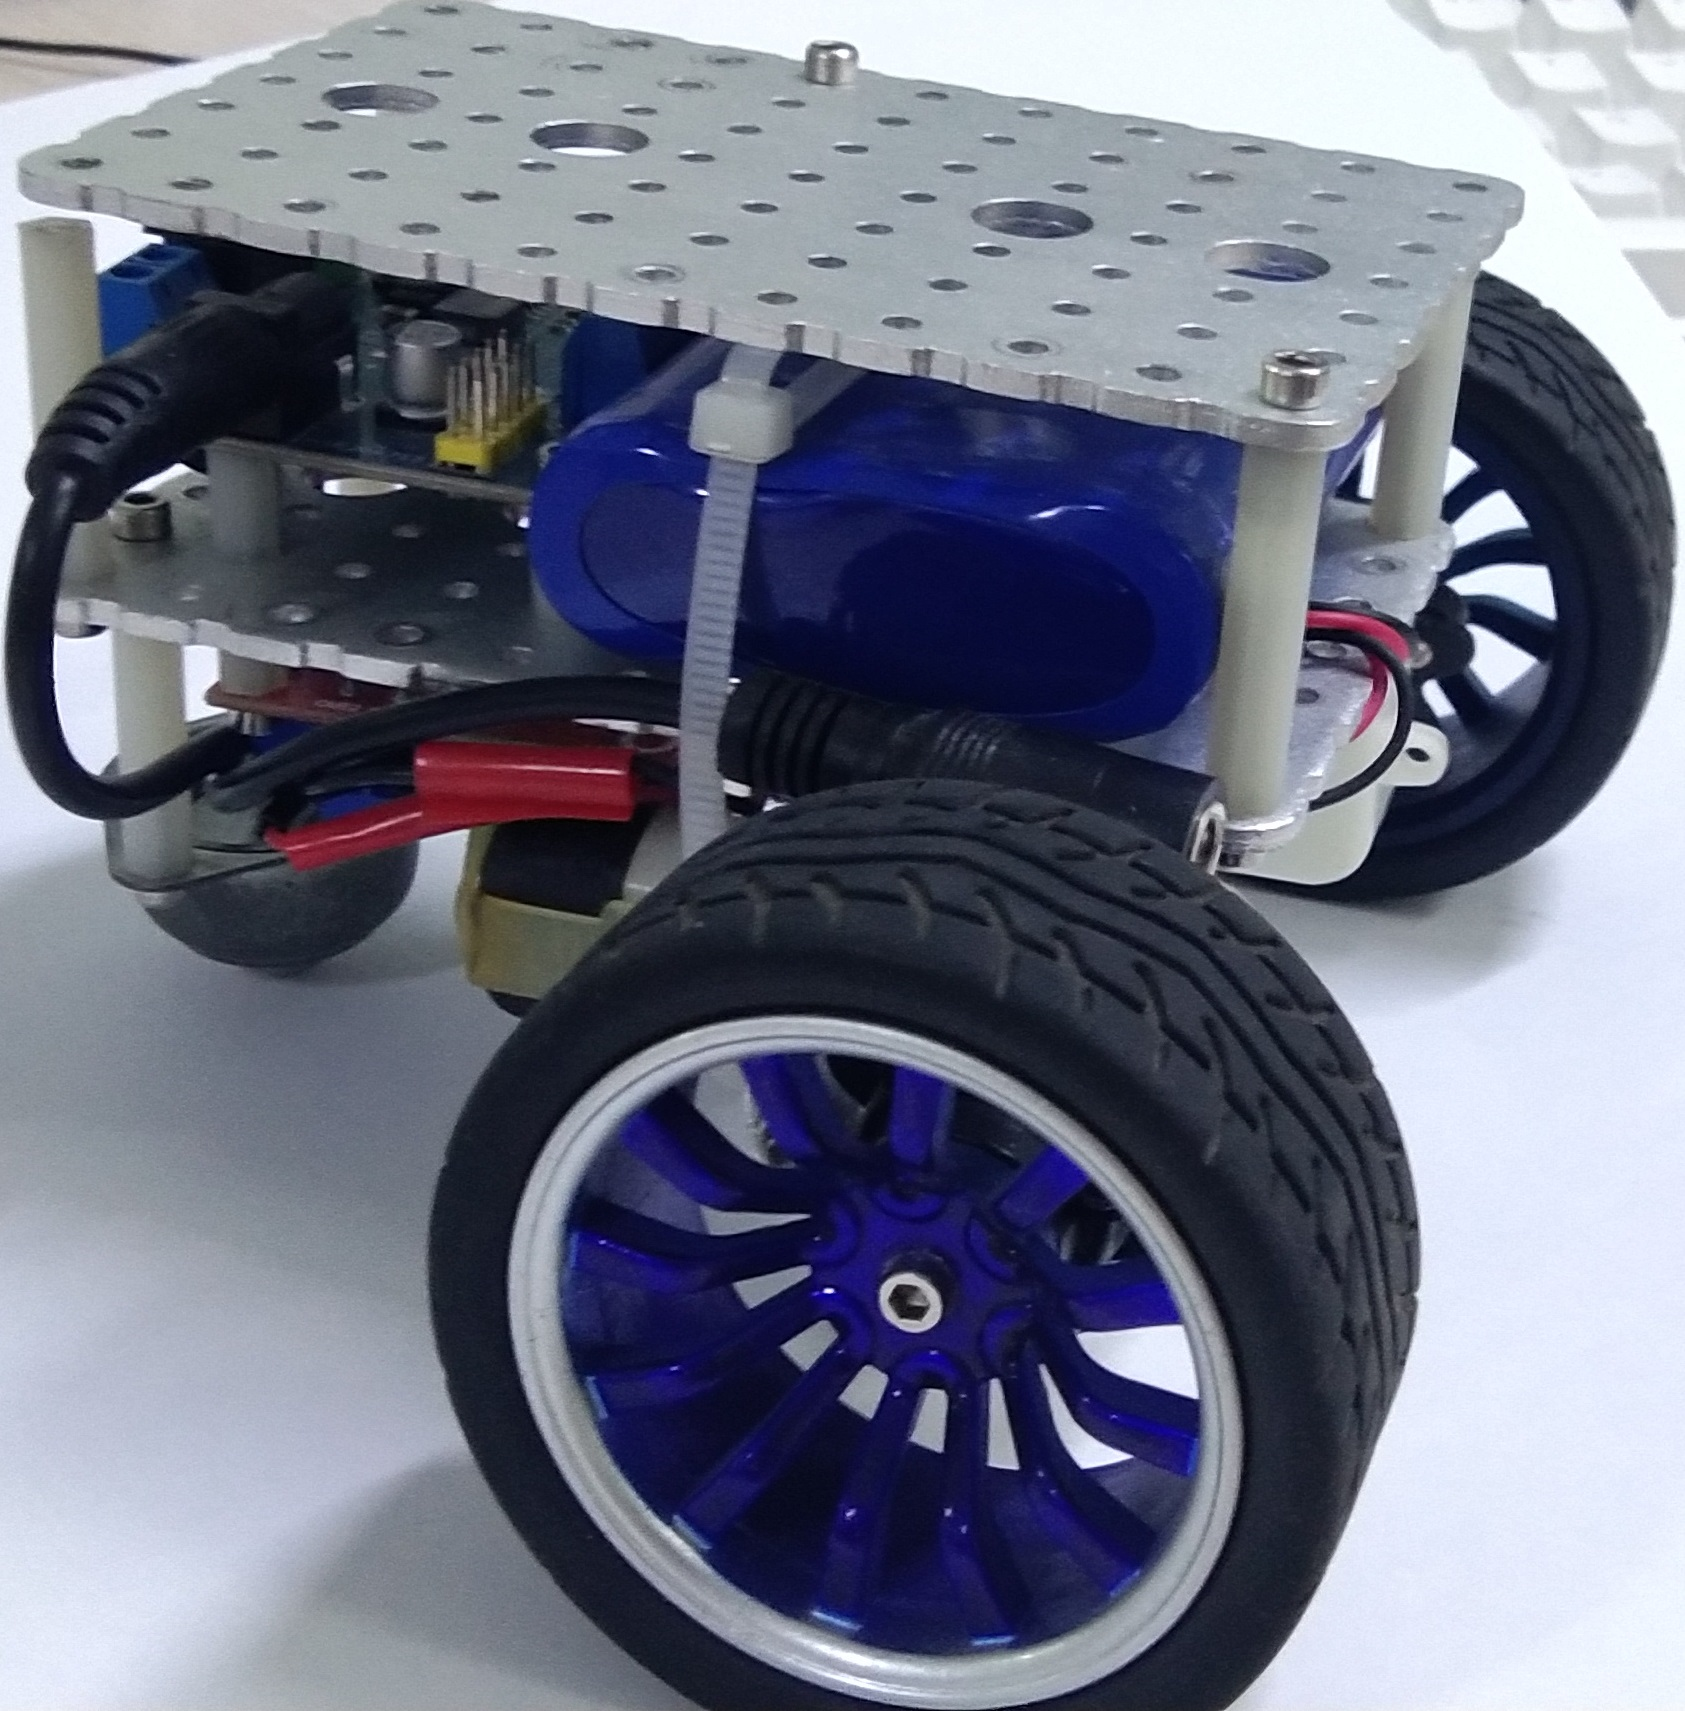
\includegraphics[width=0.5\linewidth]{AGV骨架.jpg}
    \caption{AGV骨架.}
    \label{fig:AGVgj}
\end{figure}

\subsection{xx}
三维结构图如\autoref{fig:zj}(a)所示。图如\autoref{fig:zj}(b)所示。如\autoref{fig:zj}(c)所示。
\begin{figure}[H]
    \centering
    \subfloat[摄像头支架]{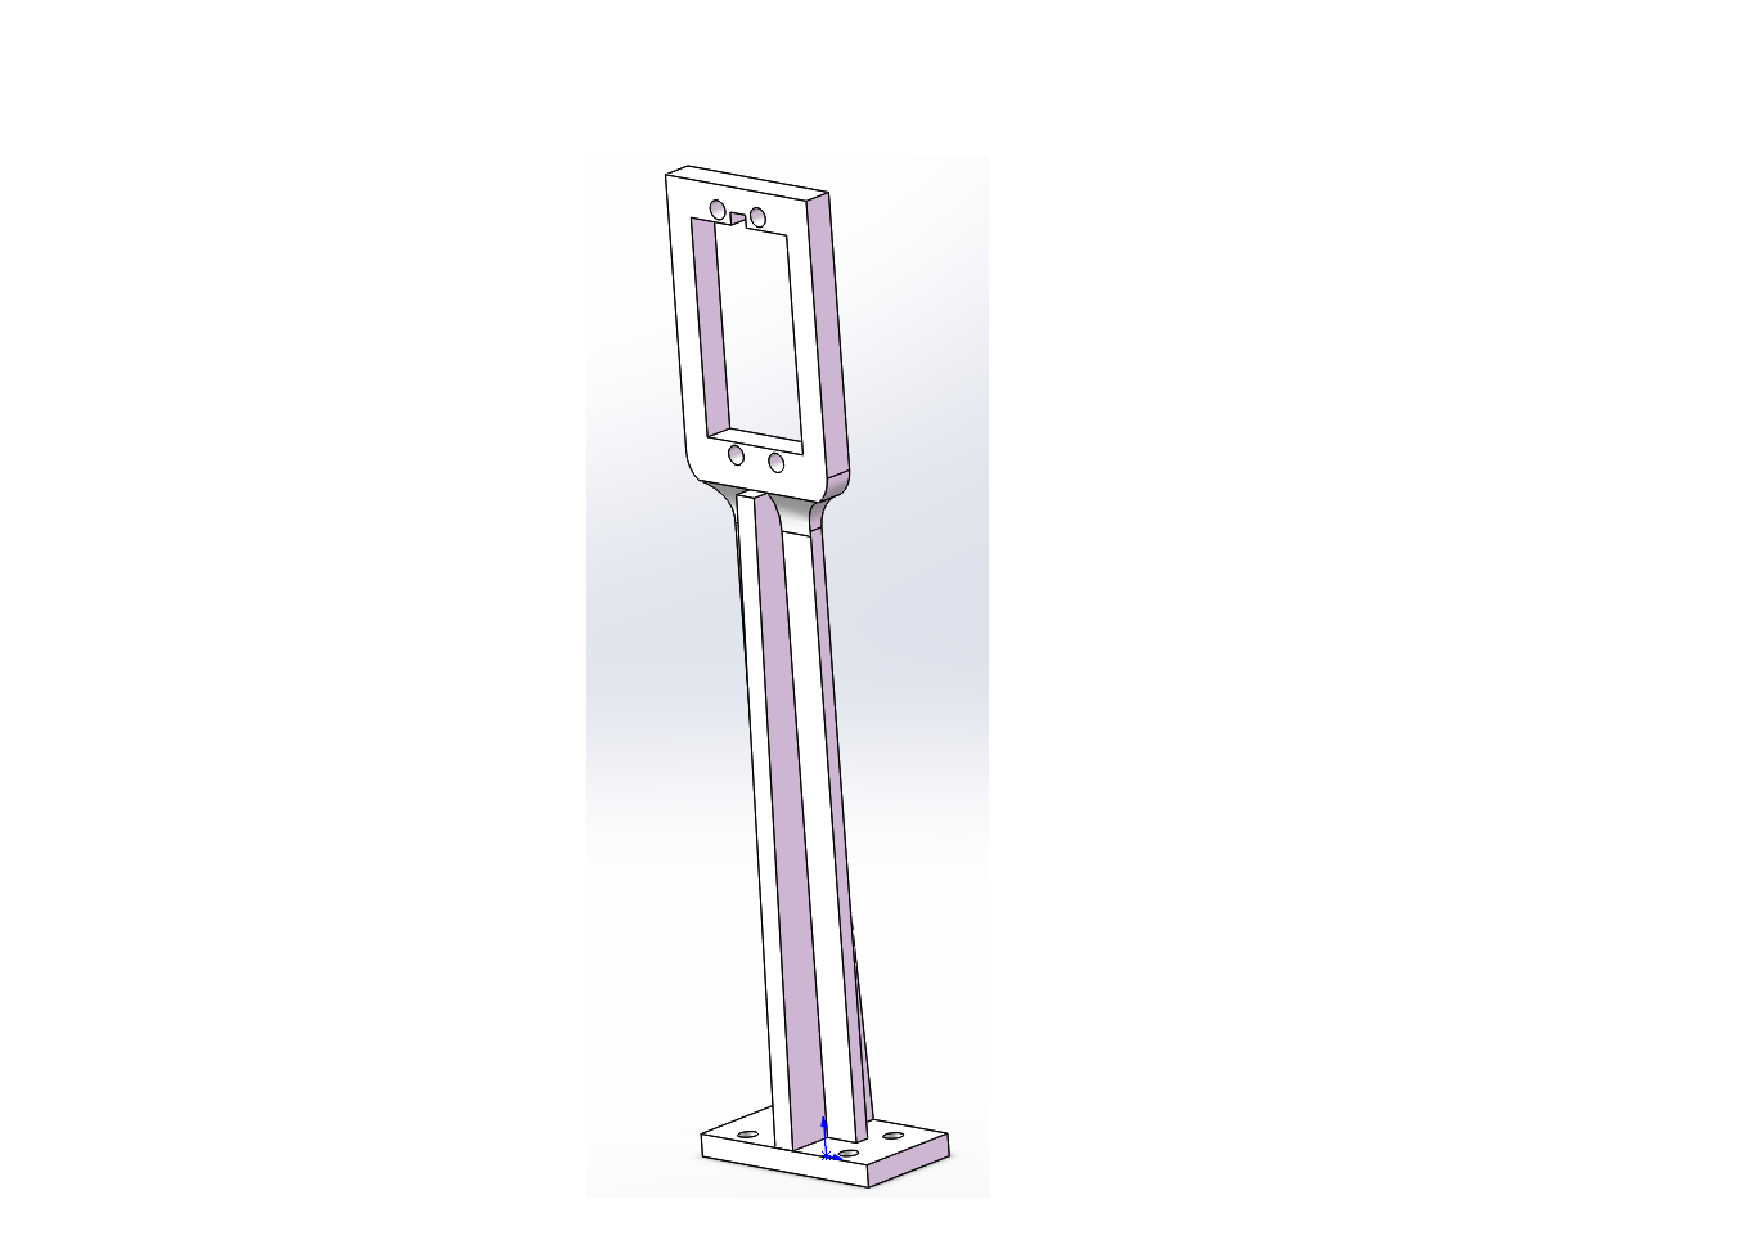
\includegraphics[height=60mm]{摄像头支架.PDF}}
    \hfill
    \subfloat[照相机联轴器]{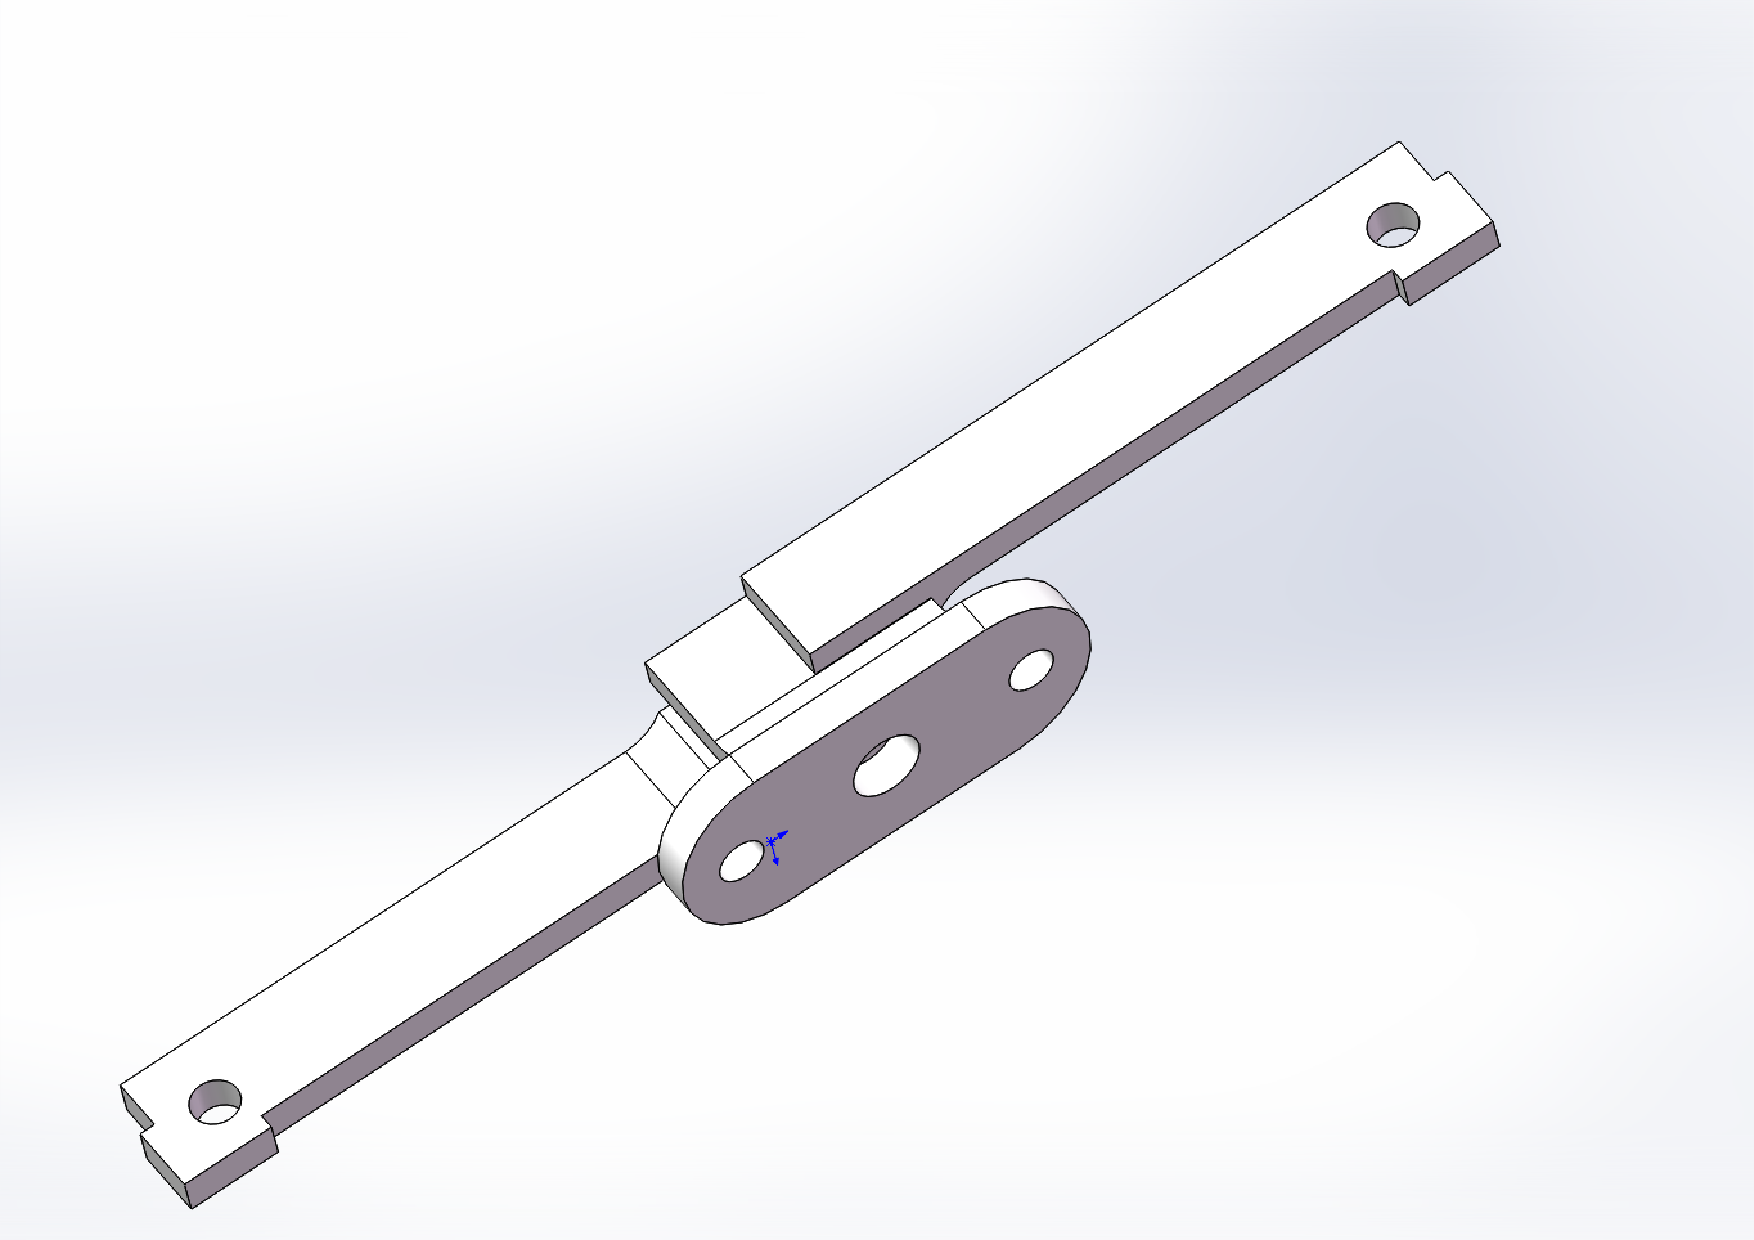
\includegraphics[height=50mm]{照相机联轴器.PDF}}
    \hfill
    \subfloat[支架实体]{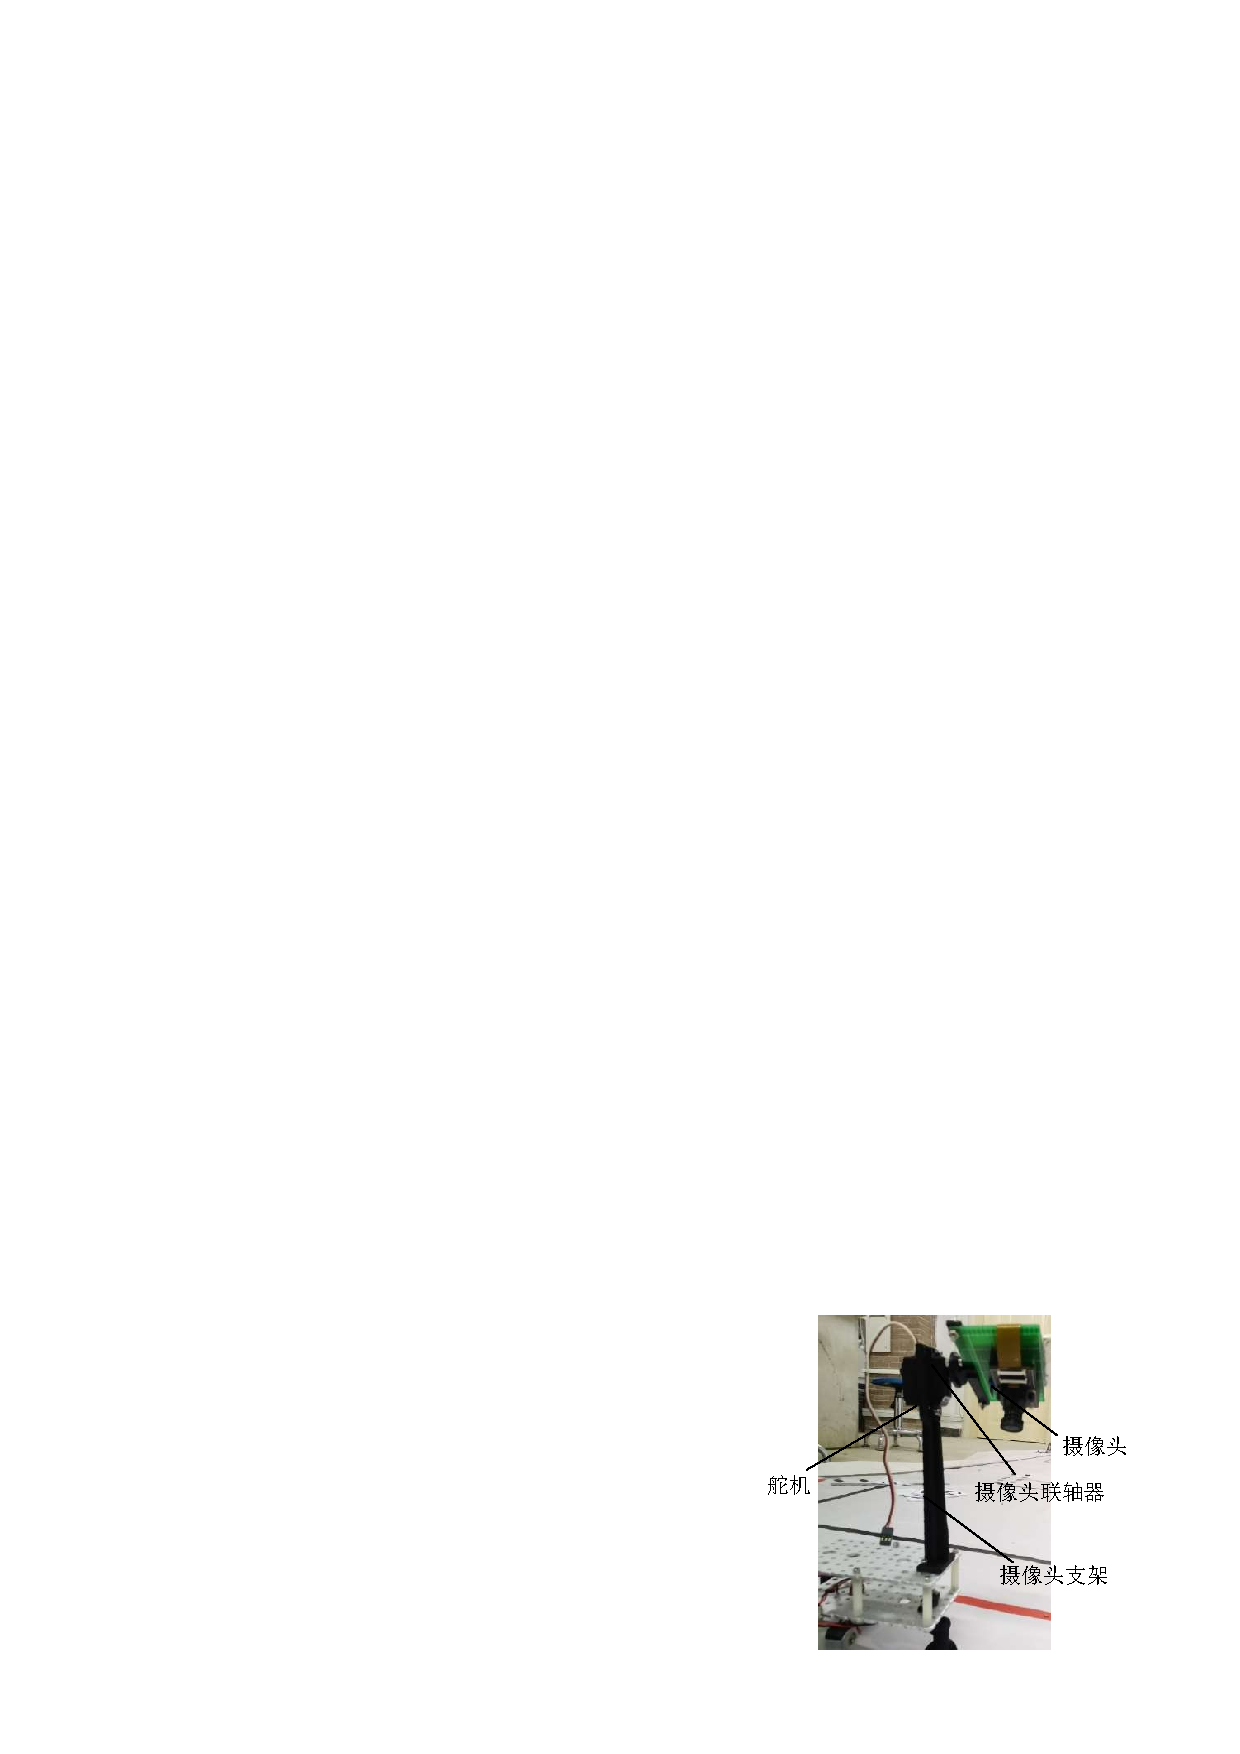
\includegraphics[height=50mm]{支架实体.pdf}}
    \caption{摄像头支架.}
    \label{fig:zj}
  \end{figure}

引脚定义如\autoref{tab:yjdy}
\begin{table}[H]
    \centering
    \small
    \caption{W25Q16引脚定义.}
    \label{tab:yjdy}
    \begin{tabular}{cccc}
    \toprule
    引脚编号 & 引脚名称       & I/O & 功能             \\ \midrule
    1    & /CS        & I   & 片选端输入          \\
    2    & DO(IO1)    & I/O & 数据输出(数据输入输出1)  \\
    3    & /WP(IO2)   & I/O & 写保护输入(数据输入输出2) \\
    4    & GND        & -   & 地              \\
    5    & DI(IO0)    & I/O & 数据输入(数据输入输出0)  \\
    6    & CLK        & I   & 串行时钟输入         \\
    7    & /HOLD(IO3) & I/O & 保持端输入(数据输入输出3) \\
    8    & VCC        & -   & 电源             \\ \bottomrule
\end{tabular}
\end{table}
芯片手册给出的电源域详细说明\footnote{注意:组A、B、C 之间的IO 电源相互不互联,电压可以不一致;相同组内的IO 电源互联,电压一致。}


\section{本章小结}
本章主要...
